\section{Results}\label{sec:results}

All results use LightGBM as base model and nominal level 0.90 unless stated otherwise. A negative CE contrast favours the first method. Exploratory results carry no confirmatory claim, ``significant'' is not used outside the pre-specified family, and unadjusted $p$-values are descriptive. Sections~\ref{sec:explor} to~\ref{sec:width} concern the design and first hold-out panels, Section~\ref{sec:panel2} the extension, and Section~\ref{sec:ablation} the ablations and Chronos.

\subsection{Calibration of adaptive methods against the baselines}\label{sec:explor}

The exploratory run covers 13 units, origins from 2000-01 and target months to 2025-06 at warm-up 48. Pooled coverage at $h=1,3,6,12$ is 0.946, 0.937, 0.917 and 0.864 for split conformal, 0.917, 0.916, 0.900 and 0.869 for rolling, and 0.908, 0.906, 0.899 and 0.864 for ACI (2024, 1972, 1894 and 1738 unit-months; the full table is in the Appendix and Figure~\ref{fig:coverage_h} shows all panels). Split conformal over-covers at short horizons. Bootstrap 95 percent intervals are wide: for ACI \ci{0.879}{0.930} at $h=3$ and \ci{0.797}{0.914} at $h=12$.

\begin{figure}[t]
\centering
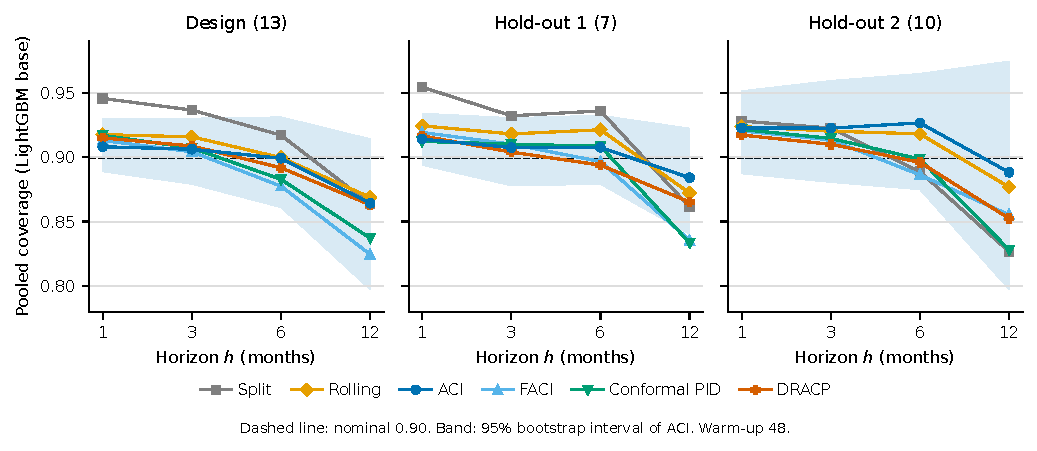
\includegraphics[width=\linewidth]{figures/fig_coverage_h.pdf}
\caption{Pooled empirical coverage by horizon and interval method for each panel (LightGBM base), against the nominal level 0.90.}
\label{fig:coverage_h}
\end{figure}

Tables~\ref{tab:ce_expl} and~\ref{tab:ce_ho1} give the calibration error. In the exploratory data the CE of ACI at $h=1,3,6,12$ is 0.013, 0.014, 0.035 and 0.069, against 0.038, 0.036, 0.050 and 0.091 for rolling and 0.071, 0.060, 0.069 and 0.139 for split. On the first hold-out panel it is 0.020, 0.020, 0.025 and 0.048 for ACI, 0.029, 0.036, 0.032 and 0.086 for rolling, and 0.056, 0.050, 0.053 and 0.119 for split.

\begin{table}[t]
\centering
\caption{Calibration error by base model, interval method and horizon, design panel (13 countries, exploratory, warm-up 48).}
\label{tab:ce_expl}
\small
\fittable{\begin{tabular}{llrrrr}
\toprule
Base model & Interval & $h{=}1$ & $h{=}3$ & $h{=}6$ & $h{=}12$ \\
\midrule
LightGBM & Split & 0.071 & 0.060 & 0.069 & 0.139 \\
 & Rolling & 0.038 & 0.036 & 0.050 & 0.091 \\
 & ACI & 0.013 & 0.014 & 0.035 & 0.069 \\
 & FACI & 0.014 & 0.018 & 0.041 & 0.101 \\
 & Conformal PID & 0.030 & 0.033 & 0.059 & 0.105 \\
 & DRACP & 0.016 & 0.016 & 0.033 & 0.074 \\
\midrule
ARIMA & Split & 0.064 & 0.064 & 0.098 & 0.148 \\
 & Rolling & 0.031 & 0.032 & 0.058 & 0.096 \\
 & ACI & 0.010 & 0.015 & 0.026 & 0.079 \\
 & FACI & 0.017 & 0.023 & 0.029 & 0.102 \\
 & Conformal PID & 0.027 & 0.020 & 0.046 & 0.099 \\
 & DRACP & 0.012 & 0.015 & 0.021 & 0.072 \\
 & Native & 0.047 & 0.066 & 0.089 & 0.137 \\
\midrule
Naive B & Split & 0.057 & 0.069 & 0.073 & 0.171 \\
 & Rolling & 0.031 & 0.035 & 0.043 & 0.100 \\
 & ACI & 0.012 & 0.016 & 0.024 & 0.057 \\
 & FACI & 0.017 & 0.018 & 0.039 & 0.124 \\
 & Conformal PID & 0.025 & 0.021 & 0.036 & 0.113 \\
 & DRACP & 0.017 & 0.017 & 0.028 & 0.071 \\
\midrule
ETS & Native & 0.044 & 0.051 & 0.064 & 0.116 \\
\bottomrule
\end{tabular}
}
\end{table}

\begin{table}[t]
\centering
\caption{Calibration error by base model, interval method and horizon, first hold-out panel (7 countries, warm-up 48).}
\label{tab:ce_ho1}
\small
\fittable{\begin{tabular}{llrrrr}
\toprule
Base model & Interval & $h{=}1$ & $h{=}3$ & $h{=}6$ & $h{=}12$ \\
\midrule
LightGBM & Split & 0.056 & 0.050 & 0.053 & 0.119 \\
 & Rolling & 0.029 & 0.036 & 0.032 & 0.086 \\
 & ACI & 0.020 & 0.020 & 0.025 & 0.048 \\
 & FACI & 0.023 & 0.023 & 0.013 & 0.070 \\
 & Conformal PID & 0.024 & 0.028 & 0.021 & 0.079 \\
 & DRACP & 0.021 & 0.019 & 0.022 & 0.047 \\
\midrule
ARIMA & Split & 0.067 & 0.065 & 0.061 & 0.106 \\
 & Rolling & 0.039 & 0.043 & 0.040 & 0.069 \\
 & ACI & 0.014 & 0.013 & 0.024 & 0.040 \\
 & FACI & 0.019 & 0.010 & 0.029 & 0.084 \\
 & Conformal PID & 0.029 & 0.037 & 0.034 & 0.083 \\
 & DRACP & 0.020 & 0.011 & 0.027 & 0.051 \\
 & Native & 0.053 & 0.058 & 0.062 & 0.073 \\
\midrule
Naive B & Split & 0.063 & 0.049 & 0.135 & 0.175 \\
 & Rolling & 0.039 & 0.030 & 0.061 & 0.052 \\
 & ACI & 0.015 & 0.021 & 0.030 & 0.032 \\
 & FACI & 0.026 & 0.020 & 0.036 & 0.079 \\
 & Conformal PID & 0.030 & 0.027 & 0.050 & 0.070 \\
 & DRACP & 0.024 & 0.024 & 0.032 & 0.055 \\
\midrule
ETS & Native & 0.056 & 0.035 & 0.048 & 0.053 \\
\bottomrule
\end{tabular}
}
\end{table}

The exploratory contrasts of the primary family at warm-up 48 are ACI minus rolling $-2.2$~pp at $h=3$ and $-1.5$~pp at $h=6$, with unadjusted $p$-values 0.030 and 0.020 but Holm-adjusted 0.090 and 0.078, so neither survives the family correction. ACI minus split (secondary) was $-4.6$~pp at $h=3$ (95\% interval \ci{-5.0}{-1.4}, unadjusted $p=0.001$) and $-3.4$~pp at $h=6$ ($p=0.0025$). DRACP minus ACI was $+0.2$~pp and $-0.2$~pp, within noise. Equivalence within 2~pp was shown at warm-up 48 (maximum one-sided $p$ 0.0085 and 0.0135) and not at warm-up 96 (0.128 and 0.146); at warm-up 96 DRACP was wider than ACI, with a Winkler score higher by 33.2 percent at $h=3$ (\ci{12.1}{75.9}, unadjusted $p=0.049$), so equivalence in the exploratory data is not stable across warm-ups. Per-country split coverage at $h=3$ ranges from 0.822 (Peru) to 1.000 (Indonesia), while ACI ranges from 0.886 to 0.934. At $h=12$ pooled coverage is below nominal for every method (0.825 to 0.869) and the adaptive methods do not repair it; the bootstrap intervals of ACI, DRACP, rolling and split include 0.90 (upper limits 0.915 to 0.920), those of FACI and conformal PID do not (0.876, 0.897). Mean absolute error relative to naive B was 0.74 (ARIMA), 0.72 (ETS) and 0.74 (LightGBM) at $h=3$ and 0.86, 0.93 and 0.91 at $h=12$.

\subsection{First hold-out panel and the decision rules R1--R5}\label{sec:holdout}

The hold-out run covers 7 countries and target months 2009-02 to 2026-06, with 205 and 199 pooled months at $h=3$ and $h=6$ in run A (warm-up 48) and 157 and 151 in run B (warm-up 96); run A has 1163, 1135, 1093 and 1009 unit-months at $h=1,3,6,12$. Pooled coverage in run A at $h=1,3,6,12$ is 0.954, 0.932, 0.936 and 0.861 for split, 0.924, 0.918, 0.921 and 0.872 for rolling, and 0.914, 0.907, 0.908 and 0.884 for ACI (all methods in the Appendix). At $h=12$ the pooled coverage of every method is below 0.90 (0.833 to 0.884); the bootstrap upper limits of ACI, DRACP, rolling and split (0.901 to 0.923) do not exclude 0.90, those of FACI and conformal PID (0.885, 0.884) do. Table~\ref{tab:contrasts} gives the primary contrasts of all panels, and the rules are applied as pre-specified.

\begin{table}[t]
\centering
\caption{Primary-family calibration-error contrasts by panel and base model: $T$ (pp of CE), 95\% block-bootstrap interval, Holm-adjusted $p$, minimum detectable difference (MDE) and verdict under the power rule. ``Inconclusive'' with an undefined MDE is not evidence of no effect.}
\label{tab:contrasts}
\small
\fittable{\begin{tabular}{llcllrrrl}
\toprule
Panel & Base & $h$ & Contrast & $T$ (pp) & 95\% CI & Holm $p$ & MDE (pp) & Verdict \\
\midrule
Design (13) & LightGBM & 3 & ACI $-$ rolling & $-$2.2 & [$-$2.7, +0.1] & 0.090 & -- & Inconclusive \\
 &  & 6 & ACI $-$ rolling & $-$1.5 & [$-$2.1, $-$0.1] & 0.078 & -- & Inconclusive \\
 &  & 3 & DRACP $-$ ACI & +0.2 & [$-$1.2, +1.0] & 1.000 & -- & Inconclusive \\
 &  & 6 & DRACP $-$ ACI & $-$0.2 & [$-$2.0, +1.3] & 1.000 & -- & Inconclusive \\
\midrule
Hold-out 1 (7) & LightGBM & 3 & ACI $-$ rolling & $-$1.6 & [$-$3.0, +0.5] & 0.350 & -- & Inconclusive \\
 &  & 6 & ACI $-$ rolling & $-$0.7 & [$-$2.8, +1.3] & 1.000 & -- & Inconclusive \\
 &  & 3 & DRACP $-$ ACI & $-$0.1 & [$-$1.2, +0.9] & 1.000 & -- & Inconclusive \\
 &  & 6 & DRACP $-$ ACI & $-$0.3 & [$-$1.4, +1.7] & 1.000 & -- & Inconclusive \\
\midrule
Design (13), from 2010 & LightGBM & 3 & ACI $-$ rolling & $-$2.1 & [$-$2.9, +0.5] & 0.216 & -- & Inconclusive \\
 &  & 6 & ACI $-$ rolling & $-$2.0 & [$-$3.1, +0.5] & 0.216 & -- & Inconclusive \\
 &  & 3 & DRACP $-$ ACI & $-$0.5 & [$-$1.6, +1.3] & 0.654 & -- & Inconclusive \\
 &  & 6 & DRACP $-$ ACI & +1.9 & [$-$1.0, +5.5] & 0.654 & -- & Inconclusive \\
\midrule
Design (13), from 2010 & Chronos & 3 & ACI $-$ rolling & $-$1.9 & [$-$2.3, +0.9] & 0.363 & -- & Inconclusive \\
 &  & 6 & ACI $-$ rolling & $-$2.0 & [$-$2.5, +0.8] & 0.358 & -- & Inconclusive \\
 &  & 3 & DRACP $-$ ACI & +0.0 & [$-$1.4, +1.3] & 0.982 & -- & Inconclusive \\
 &  & 6 & DRACP $-$ ACI & +2.4 & [$-$0.6, +5.9] & 0.363 & -- & Inconclusive \\
\midrule
Hold-out 1 (7), from 2010 & LightGBM & 3 & ACI $-$ rolling & $-$2.4 & [$-$5.5, +0.7] & 0.496 & -- & Inconclusive \\
 &  & 6 & ACI $-$ rolling & $-$4.7 & [$-$9.6, +0.5] & 0.390 & -- & Inconclusive \\
 &  & 3 & DRACP $-$ ACI & $-$0.8 & [$-$2.2, +1.2] & 0.656 & -- & Inconclusive \\
 &  & 6 & DRACP $-$ ACI & +0.2 & [$-$2.2, +1.4] & 0.904 & -- & Inconclusive \\
\midrule
Hold-out 1 (7), from 2010 & Chronos & 3 & ACI $-$ rolling & $-$1.3 & [$-$4.9, +0.7] & 1.000 & -- & Inconclusive \\
 &  & 6 & ACI $-$ rolling & $-$2.0 & [$-$4.5, +1.4] & 0.962 & -- & Inconclusive \\
 &  & 3 & DRACP $-$ ACI & $-$0.2 & [$-$2.0, +1.2] & 1.000 & -- & Inconclusive \\
 &  & 6 & DRACP $-$ ACI & +0.2 & [$-$2.5, +4.3] & 1.000 & -- & Inconclusive \\
\midrule
Hold-out 2 (10) & LightGBM & 3 & ACI $-$ rolling & $-$3.7 & [$-$5.1, $-$0.7] & 0.008 & 3.2 & Met \\
 &  & 6 & ACI $-$ rolling & $-$3.5 & [$-$4.9, +0.5] & 0.159 & 6.1 & Not met \\
 &  & 3 & DRACP $-$ ACI & $-$1.0 & [$-$2.0, +0.9] & 0.321 & -- & Inconclusive \\
 &  & 6 & DRACP $-$ ACI & $-$1.3 & [$-$2.7, +2.0] & 0.337 & -- & Inconclusive \\
\midrule
Hold-out 2 (10) & ARIMA & 3 & ACI $-$ rolling & $-$3.2 & [$-$3.6, $-$1.1] & 0.004 & 3.2 & Met \\
 &  & 6 & ACI $-$ rolling & $-$3.1 & [$-$3.9, $-$0.5] & 0.030 & 3.5 & Met \\
 &  & 3 & DRACP $-$ ACI & $-$1.5 & [$-$2.4, +0.8] & 0.199 & -- & Inconclusive \\
 &  & 6 & DRACP $-$ ACI & $-$1.8 & [$-$3.4, +0.7] & 0.199 & -- & Inconclusive \\
\midrule
Hold-out 2 (10) & Naive B & 3 & ACI $-$ rolling & $-$4.1 & [$-$4.9, $-$1.5] & 0.004 & 1.2 & Met \\
 &  & 6 & ACI $-$ rolling & $-$3.4 & [$-$4.7, $-$0.4] & 0.039 & 3.5 & Met \\
 &  & 3 & DRACP $-$ ACI & $-$1.2 & [$-$2.3, +0.9] & 0.422 & -- & Inconclusive \\
 &  & 6 & DRACP $-$ ACI & $-$1.8 & [$-$3.3, +2.5] & 0.422 & -- & Inconclusive \\
\midrule
Hold-out 2 (10) & Chronos & 3 & ACI $-$ rolling & $-$3.3 & [$-$4.0, $-$0.3] & 0.036 & -- & Inconclusive \\
 &  & 6 & ACI $-$ rolling & $-$2.5 & [$-$3.6, +0.1] & 0.088 & 6.6 & Not met \\
 &  & 3 & DRACP $-$ ACI & $-$0.5 & [$-$1.8, +1.3] & 0.454 & -- & Inconclusive \\
 &  & 6 & DRACP $-$ ACI & $-$1.2 & [$-$2.2, +1.3] & 0.443 & -- & Inconclusive \\
\bottomrule
\end{tabular}
}
\end{table}

\paragraph{R1 (ACI better calibrated than split): not met in the primary run; met at warm-up 96, a sensitivity run that is not promoted.} At warm-up 48 ACI minus split was $-3.0$~pp ($p=0.054$) at $h=3$ and $-2.8$~pp ($p=0.092$) at $h=6$, with intervals \ci{-5.4}{+0.5} and \ci{-3.9}{+1.2} that include zero; at warm-up 96 it was $-4.1$~pp ($p=0.018$) and $-5.9$~pp ($p=0.0025$). The direction replicates in both runs. Applying Holm over the two horizons (the result files have no Holm column for this secondary contrast) gives 0.108 at both horizons at warm-up 48 and 0.018 and 0.005 at warm-up 96; at warm-up 48 the rule fails with unadjusted as well as adjusted $p$-values, so the verdict for the primary configuration is ``not met'', and warm-up 96 was not promoted because R1 holds there.

\paragraph{R2 (ACI improves on rolling): not shown on this panel (MDE undefined, inconclusive).} Holm $p$ was 0.35 ($h=3$) and 1.0 ($h=6$) at warm-up 48 and 0.59 and 0.99 at warm-up 96, with point estimates $-1.6$ and $-0.7$~pp at warm-up 48. On the Winkler score ACI was 1.0 percent lower than rolling at $h=3$ (\ci{-7.1}{+4.1}) and 5.3 percent higher at $h=6$ (\ci{+1.4}{+8.1}, unadjusted $p=0.005$); these contrasts are descriptive. The second hold-out panel gives a different result (Section~\ref{sec:panel2}); the results are not combined.

\paragraph{R3 (DRACP against ACI): inconclusive.} Equivalence within 2~pp was shown at warm-up 48 (TOST $p$ 0.0005 at $h=3$ and 0.047 at $h=6$) and not at warm-up 96 (0.062 and 0.355). The wording ``no advantage, equivalent within 2~pp'' requires both warm-ups, so the verdict is inconclusive, and DRACP minus ACI is not negative with Holm $p$ below 0.05 at either warm-up, so ``DRACP better'' is not supported either. The 2~pp margin is of the size of the calibration error of ACI itself, so even the equivalence verdict at warm-up 48 is weak, and because the MDE of these contrasts is undefined, R5 classifies them as inconclusive whatever the TOST result.

\paragraph{R4 (delayed feedback explains the $h=12$ shortfall; ACI at least $+3$~pp): not met.} ACI coverage at $h=12$ was 0.884 delayed and 0.908 instant, a difference of $+2.4$~pp (Section~\ref{sec:feedback}).

\paragraph{R5 (power): all four primary contrasts are inconclusive.} The MDE is undefined on the full hold-out sample at both warm-ups, because the baseline calibration error is too small for a 10~pp improvement to be attainable. On random 15-month windows of the hold-out data the median MDE is 2.6 to 3.1~pp, but 63 to 68 percent of windows have an undefined MDE; it is also undefined in the exploratory data at warm-up 48. None of the four primary contrasts supports a conclusion.

\paragraph{What the hold-out result supports.} A direction in favour of adaptive methods over one-shot calibration, replicated in the exploratory data and at both warm-ups, with intervals that include zero at the primary warm-up. It does not support the statements that adaptivity helps beyond a rolling window or that DRACP is better than ACI. At $h=12$ the standard deviation of coverage across units is 0.058 for ACI and 0.152 for split.

\subsection{Robustness (S1, S2) and width}\label{sec:width}

The robustness analyses S1--S5 were written after the hold-out result and before they were computed, use only existing intervals and do not replace R1--R5. In S1 (leave one country out, LightGBM, warm-up 48; Appendix Table~\ref{tab:loo}) no removal flips the sign of ACI minus split in either sample (ranges $-5.1$ to $-2.1$~pp over both horizons and samples), so the advantage over a calibration done once does not depend on any single country. ACI minus rolling is negative for almost every removal (one flip in seven at $h=6$ on the hold-out panel, range $-1.3$ to $+0.1$~pp), but its interval includes zero in the primary run, so ``not shown'' stands. The DRACP minus ACI estimates sit at zero and change sign when one or two countries are removed. S2 (other base models; Appendix Table~\ref{tab:s2full}) is in Section~\ref{sec:basemodel}.

Three width statistics must be kept apart, and they do not give the same answer (Appendix Table~\ref{tab:width}). \emph{Median width relative to rolling:} at $h=1$ and $h=3$ ACI, DRACP and FACI have a lower median width in both samples (ACI 0.91 and 0.93 in the exploratory data, 0.84 and 0.90 on the first hold-out panel). \emph{Pooled mean width:} for ACI at $h=3$ it is larger than rolling's in both samples (4.28 against 3.95 exploratory, 5.856 against 5.786 hold-out), which indicates heavy tails in the adaptive widths; DRACP is wider than ACI at $h=3$ (4.97 against 4.28) and $h=12$ (24.3 against 15.5) in the exploratory data, but not on the hold-out panel, where its Winkler score at warm-up 96 was 5.8 percent lower than ACI's at $h=3$ (\ci{-14.2}{+3.3}, $p=0.18$). \emph{Winkler score:} the ratio to rolling for ACI, DRACP and FACI at $h=1$ and $h=3$ is 0.94 to 0.99 on the hold-out panel and 0.99 to 1.16 in the exploratory data (ACI 1.06 and DRACP 1.16 at $h=3$; ACI 6.3 percent higher than rolling at $h=3$, \ci{0.3}{19.4}, unadjusted $p=0.15$), and at $h=6$ and $h=12$ it exceeds 1 in most cells of both samples (up to 1.38). No efficiency advantage is established; at long horizons the better calibration is paid for with width or interval score.

\subsection{Second hold-out panel (extension)}\label{sec:panel2}

The second panel has 10 countries and 198 months from 2010-01 (89 and 83 pooled months at $h=3$ and $h=6$ at warm-up 48; 41 and 35 at warm-up 96), four base models and a Holm family of four tests per base model. Warm-up 48 is primary. Table~\ref{tab:ce_ho2} gives the CE: at $h=3$ and $h=6$ ACI has 0.033 and 0.045 for LightGBM, rolling 0.070 and 0.080, split 0.104 and 0.125, and the native ARIMA intervals 0.058 and 0.084. On the first hold-out panel the CE of the rolling window at $h=3$ and $h=6$ is 0.036 and 0.032, against 0.066 to 0.090 and 0.075 to 0.087 here; this is a descriptive observation, and its relation to the results below was not tested.

\begin{table}[t]
\centering
\caption{Calibration error by interval method, horizon and base model, second hold-out panel (10 countries, warm-up 48).}
\label{tab:ce_ho2}
\small
\fittable{\begin{tabular}{llrrrr}
\toprule
Base model & Interval & $h{=}1$ & $h{=}3$ & $h{=}6$ & $h{=}12$ \\
\midrule
LightGBM & Split & 0.084 & 0.104 & 0.125 & 0.154 \\
 & Rolling & 0.050 & 0.070 & 0.080 & 0.089 \\
 & ACI & 0.032 & 0.033 & 0.045 & 0.072 \\
 & FACI & 0.024 & 0.027 & 0.042 & 0.079 \\
 & Conformal PID & 0.043 & 0.051 & 0.070 & 0.103 \\
 & DRACP & 0.023 & 0.023 & 0.032 & 0.078 \\
\midrule
ARIMA & Split & 0.086 & 0.098 & 0.111 & 0.136 \\
 & Rolling & 0.053 & 0.066 & 0.084 & 0.089 \\
 & ACI & 0.026 & 0.034 & 0.052 & 0.074 \\
 & FACI & 0.033 & 0.023 & 0.035 & 0.075 \\
 & Conformal PID & 0.037 & 0.047 & 0.073 & 0.105 \\
 & DRACP & 0.017 & 0.019 & 0.034 & 0.071 \\
 & Native & 0.052 & 0.058 & 0.084 & 0.132 \\
\midrule
Naive B & Split & 0.079 & 0.122 & 0.105 & 0.188 \\
 & Rolling & 0.057 & 0.090 & 0.087 & 0.110 \\
 & ACI & 0.023 & 0.049 & 0.052 & 0.089 \\
 & FACI & 0.024 & 0.049 & 0.055 & 0.082 \\
 & Conformal PID & 0.054 & 0.073 & 0.074 & 0.122 \\
 & DRACP & 0.020 & 0.037 & 0.034 & 0.087 \\
\midrule
Chronos & Split & 0.078 & 0.109 & 0.107 & 0.111 \\
 & Rolling & 0.048 & 0.067 & 0.075 & 0.078 \\
 & ACI & 0.028 & 0.034 & 0.050 & 0.062 \\
 & FACI & 0.017 & 0.031 & 0.041 & 0.088 \\
 & Conformal PID & 0.040 & 0.052 & 0.073 & 0.105 \\
 & DRACP & 0.021 & 0.030 & 0.038 & 0.082 \\
\bottomrule
\end{tabular}
}
\end{table}

ACI minus split (secondary, $h=3$ and $h=6$) is $-7.0$ and $-8.0$~pp for LightGBM, $-6.4$ and $-5.8$ for ARIMA, $-7.3$ and $-5.3$ for naive B and $-7.4$ and $-5.7$ for Chronos (unadjusted $p\le 0.0045$). ACI with ARIMA has a lower CE than the native ARIMA intervals (0.034 against 0.058 at $h=3$, 0.052 against 0.084 at $h=6$); no interval for this contrast is reported for this panel.

\paragraph{R1.} At warm-up 48 R1 is met for all four base models at both horizons (unadjusted $p\le 0.0045$), by $-5.3$ to $-8.0$~pp. At warm-up 96 it is not met: LightGBM (0.048) and naive B (0.032) at $h=3$ have unadjusted $p$ below 0.05, all other cells are above, and with Holm over the two horizons none is below 0.05 (0.096 and 0.064). The direction replicates, and the threshold is met on this panel at warm-up 48 whereas on the first panel it was met only at warm-up 96.

\paragraph{R2: the result differs from the earlier panels.} At warm-up 48 R2 is met at $h=3$ for LightGBM, ARIMA and naive B (Holm 0.008, 0.004, 0.004) and at $h=6$ for ARIMA and naive B (0.030, 0.039). For Chronos at $h=3$ the Holm $p$ is 0.036 but the MDE is undefined, so under E5 that cell is inconclusive and is not counted as met; Chronos and LightGBM at $h=6$ are not met (0.088, 0.159). On the design and first hold-out panels it was not shown, with an undefined MDE (inconclusive). The earlier 20 countries re-run from 2010-01 give Holm $p$ of 0.22 to 1.0 with the MDE undefined in every cell, so those results are inconclusive under E5 and not evidence of no effect (Table~\ref{tab:contrasts}; Figure~\ref{fig:forest}). Three points should be read together. The point estimates are negative in every row; on the second panel they ($-2.5$ to $-4.1$~pp) are generally larger than on the earlier panels ($-0.7$ to $-2.4$~pp), with one exception (LightGBM on the re-run first panel at $h=6$: $-4.7$~pp, Holm $p=0.390$, \ci{-9.6}{+0.5}), so the direction does not differ between panels but its size and distance from the threshold do. ``ACI improves on a rolling window'' is reached under the pre-specified rule on one panel and not on the other two, and the data do not say why; candidate explanations (a shorter series, more volatile economies, a larger share of 198 months taken by the warm-up, a rolling window with a larger CE) were not tested. And the four base models share countries and months, so the three ``met'' cells at $h=3$ are not three independent confirmations. We do not average the panels and do not select the panel on which the rule is met.

\begin{figure}[t]
\centering
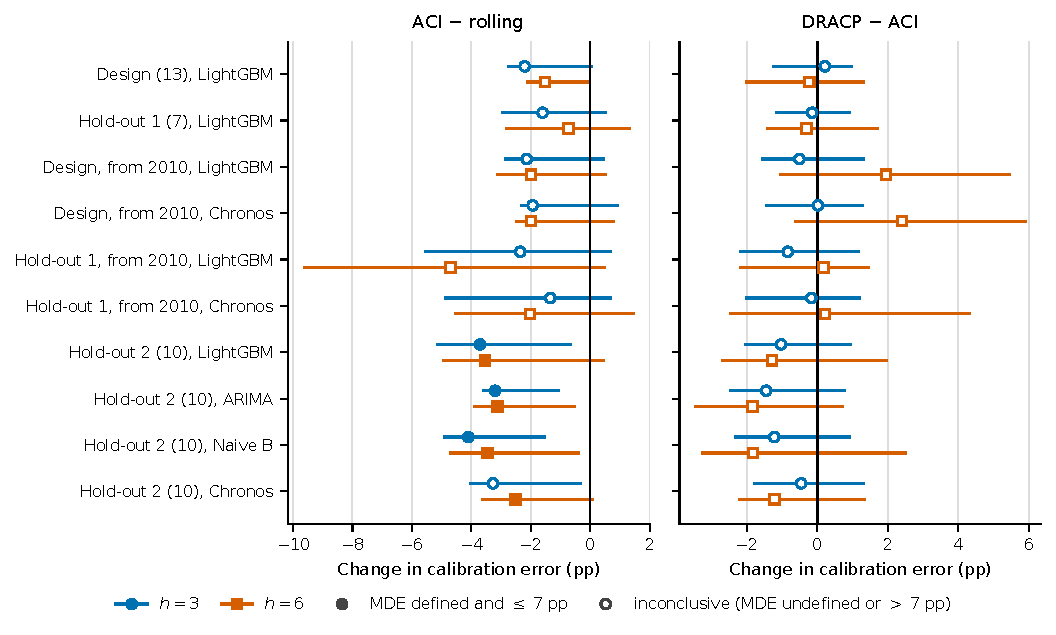
\includegraphics[width=\linewidth]{figures/fig_contrasts_forest.pdf}
\caption{Forest plot of the change in calibration error (pp) for ACI minus rolling and DRACP minus ACI, with 95\% block-bootstrap intervals. Contrasts with an undefined minimum detectable difference are inconclusive under rule E5 regardless of the interval. The panels are displayed side by side and not pooled.}
\label{fig:forest}
\end{figure}

\paragraph{Warm-up 96 shows nothing.} With 41 and 35 pooled months, ACI minus rolling is $-1.0$ to $-3.3$~pp at $h=3$ (Holm $p$ 0.147 to 1.0) and $+0.2$ (LightGBM), $+1.1$ (Chronos), $-0.5$ (ARIMA) and $-0.6$~pp (naive B) at $h=6$ (Holm $p\ge 0.59$), with the MDE undefined for every contrast; the run neither confirms nor contradicts the primary run and is not promoted.

\paragraph{R3 stays inconclusive.} At warm-up 48 DRACP has a lower CE than ACI in every cell, by 0.5 to 1.8~pp, and no difference has Holm $p$ below 0.05 (0.199 to 0.454). Equivalence within 2~pp holds only for Chronos at $h=3$ (TOST $p=0.0385$) and is not shown in the other seven cells ($p$ 0.15 to 0.76). At warm-up 96 equivalence holds for LightGBM and naive B at $h=3$ ($p=0.0375$ and 0.013) and not in the other six cells, and DRACP is better than ACI only at $h=6$ for naive B ($-2.3$~pp, Holm $p=0.002$). R3 requires the same verdict at both warm-ups, so it is not met, and under E5 every DRACP minus ACI contrast at warm-up 48 has an undefined MDE and is inconclusive whatever its $p$-value, including the equivalence of Chronos at $h=3$. The consistent tendency of DRACP towards a lower CE at warm-up 48 is a descriptive observation and not a result.

\paragraph{E5 and E2.} At warm-up 48 the MDE for ACI minus rolling is 3.2~pp ($h=3$) and 6.1~pp ($h=6$) for LightGBM, 3.2 and 3.5~pp for ARIMA, 1.2 and 3.5~pp for naive B, and 6.6~pp for Chronos at $h=6$ (undefined at $h=3$). Where R2 is not met (LightGBM and Chronos at $h=6$) the MDE of 6.1 and 6.6~pp exceeds the estimates, so ``not met'' is not evidence that the effect is absent. The conclusions about R1 and R3 do not depend on the base model, whereas the conclusion about R2 at $h=6$ does (met for ARIMA and naive B, not for LightGBM and Chronos). On the earlier 20 countries re-run from 2010-01 ACI minus split is $-3.5$ to $-9.4$~pp with unadjusted $p$ between 0.002 and 0.045. R4 was not part of the extension, and no instant-feedback run was made on the second panel.

\subsection{Ablations}\label{sec:ablation}

\paragraph{Base model.}\label{sec:basemodel} The contrasts were recomputed with ARIMA and naive B on the design and first hold-out panels (S2, Appendix Table~\ref{tab:s2full}), and Table~\ref{tab:ablation_base} gives the ablation on the second panel. ACI minus split is negative for all three base models in both samples (for naive B at $h=6$ on the first hold-out panel it is $-10.6$~pp). All DRACP minus ACI equivalence tests at warm-up 48 say ``equivalent'' within 2~pp except naive B at $h=6$ on the hold-out panel ($p=0.0515$), and at warm-up 96 on the hold-out panel most are ``not shown''. The direction ``ACI better than rolling'' holds for every base model and both samples, but unadjusted $p$-values range from 0.016 to 0.48 and none survives the correction of the pre-specified family.

\begin{table}[t]
\centering
\caption{Ablation over the base model on the second hold-out panel (warm-up 48): relative mean absolute error (naive B $=1$, all target months including flagged months), CE of ACI and of rolling, and ACI minus rolling in pp of CE with Holm $p$.}
\label{tab:ablation_base}
\small
\fittable{\begin{tabular}{lrrrrrrrr}
\toprule
& \multicolumn{2}{c}{Rel. MAE} & \multicolumn{2}{c}{CE, ACI} & \multicolumn{2}{c}{CE, rolling} & \multicolumn{2}{c}{ACI $-$ rolling, pp (Holm $p$)} \\
\cmidrule(lr){2-3}\cmidrule(lr){4-5}\cmidrule(lr){6-7}\cmidrule(lr){8-9}
Base model & $h{=}3$ & $h{=}6$ & $h{=}3$ & $h{=}6$ & $h{=}3$ & $h{=}6$ & $h{=}3$ & $h{=}6$ \\
\midrule
Naive B & 1.000 & 1.000 & 0.049 & 0.052 & 0.090 & 0.087 & $-$4.1 (0.004) & $-$3.4 (0.039) \\
ARIMA & 0.602 & 0.570 & 0.034 & 0.052 & 0.066 & 0.084 & $-$3.2 (0.004) & $-$3.1 (0.030) \\
LightGBM & 0.619 & 0.593 & 0.033 & 0.045 & 0.070 & 0.080 & $-$3.7 (0.008) & $-$3.5 (0.159) \\
Chronos & 0.586 & 0.581 & 0.034 & 0.050 & 0.067 & 0.075 & $-$3.3 (0.036) & $-$2.5 (0.088) \\
\bottomrule
\end{tabular}
}
\end{table}

\paragraph{Warm-up: 48 against 96.} Warm-up 96 is a sensitivity run applied to all methods and not promoted (Table~\ref{tab:ablation_warmup}). On the first hold-out panel ACI minus split moves from $-3.0$ and $-2.8$~pp at warm-up 48 to $-4.1$ and $-5.9$~pp at 96, which is what turns R1 from not met to met; ACI minus rolling is $-1.6$ and $-0.7$~pp at 48 and $-1.5$ and $-1.1$~pp at 96, with Holm $p$ 0.35 and 1.0 against 0.59 and 0.99. The larger warm-up removes target months (157 and 151 pooled months against 205 and 199), so the sample is also smaller, and on the second panel it leaves 41 and 35 months and shows nothing. The comparison does not select a configuration.

\begin{table}[t]
\centering
\caption{Ablation over the warm-up size: CE of ACI and rolling, ACI minus rolling and Holm $p$ at warm-up 48 (primary) and 96 (sensitivity, not promoted), by panel.}
\label{tab:ablation_warmup}
\small
\fittable{\begin{tabular}{llcrrrrrrrr}
\toprule
\multicolumn{3}{c}{} & \multicolumn{2}{c}{CE, ACI} & \multicolumn{2}{c}{CE, rolling} & \multicolumn{2}{c}{ACI $-$ rolling (pp)} & \multicolumn{2}{c}{Holm $p$} \\
\cmidrule(lr){4-5}\cmidrule(lr){6-7}\cmidrule(lr){8-9}\cmidrule(lr){10-11}
Panel & Base & $h$ & 48 & 96 & 48 & 96 & 48 & 96 & 48 & 96 \\
\midrule
Design (13) & LightGBM & 3 & 0.014 & 0.022 & 0.036 & 0.035 & $-$2.2 & $-$1.3 & 0.090 & 0.132 \\
 &  & 6 & 0.035 & 0.039 & 0.050 & 0.054 & $-$1.5 & $-$1.5 & 0.078 & 0.132 \\
\midrule
Hold-out 1 (7) & LightGBM & 3 & 0.020 & 0.027 & 0.036 & 0.042 & $-$1.6 & $-$1.5 & 0.350 & 0.592 \\
 &  & 6 & 0.025 & 0.030 & 0.032 & 0.041 & $-$0.7 & $-$1.1 & 1.000 & 0.990 \\
\midrule
Hold-out 2 (10) & LightGBM & 3 & 0.033 & 0.045 & 0.070 & 0.058 & $-$3.7 & $-$1.3 & 0.008 & 0.278 \\
 &  & 6 & 0.045 & 0.069 & 0.080 & 0.067 & $-$3.5 & +0.2 & 0.159 & 1.000 \\
\midrule
Hold-out 2 (10) & ARIMA & 3 & 0.034 & 0.043 & 0.066 & 0.053 & $-$3.2 & $-$1.0 & 0.004 & 0.340 \\
 &  & 6 & 0.052 & 0.081 & 0.084 & 0.086 & $-$3.1 & $-$0.5 & 0.030 & 0.682 \\
\midrule
Hold-out 2 (10) & Naive B & 3 & 0.049 & 0.050 & 0.090 & 0.083 & $-$4.1 & $-$3.3 & 0.004 & 0.147 \\
 &  & 6 & 0.052 & 0.071 & 0.087 & 0.077 & $-$3.4 & $-$0.6 & 0.039 & 0.593 \\
\midrule
Hold-out 2 (10) & Chronos & 3 & 0.034 & 0.048 & 0.067 & 0.063 & $-$3.3 & $-$1.5 & 0.036 & 1.000 \\
 &  & 6 & 0.050 & 0.084 & 0.075 & 0.073 & $-$2.5 & +1.1 & 0.088 & 1.000 \\
\bottomrule
\end{tabular}
}
\end{table}

\paragraph{Feedback delay.}\label{sec:feedback} At $h=12$ pooled coverage is below nominal for every method (0.83 to 0.88 on the first hold-out panel, 0.82 to 0.87 in the exploratory data), with the qualification on the bootstrap intervals given above. The diagnostic run releases each outcome at origin $+1$ instead of $+12$ (Table~\ref{tab:feedback}; paired block-bootstrap 95 percent intervals over the same cells). For ACI the change in coverage is $+4.1$~pp (\ci{1.4}{7.8}) in the exploratory data (1738 cells) and $+2.4$~pp (\ci{-0.1}{4.8}) on the hold-out panel (1009 cells); for DRACP $+4.3$ (\ci{1.4}{7.5}) and $+3.9$~pp (\ci{1.6}{6.4}); for FACI $+8.3$ (\ci{4.3}{13.6}) and $+6.4$~pp (\ci{2.5}{9.6}); for conformal PID $+5.1$ and $+5.3$~pp; for rolling $+1.3$~pp in both. R4 as pre-specified (ACI at least $+3$~pp) is not met: $+2.4$~pp, with an interval compatible with no effect and with an effect of about 5~pp. The supported statement is that delay accounts for part of the shortfall, with a size that depends on the method and sample; it is not shown that delay is, or is not, the main cause. The diagnostic is not a valid forecasting setup.

\begin{table}[t]
\centering
\caption{Ablation over the feedback delay (S3): coverage at $h=12$ with delayed and instant feedback, and the difference in pp with a 95\% paired block-bootstrap interval.}
\label{tab:feedback}
\small
\fittable{\begin{tabular}{lrrcrrc}
\toprule
& \multicolumn{3}{c}{Design (13), 1738 cells} & \multicolumn{3}{c}{Hold-out 1 (7), 1009 cells} \\
\cmidrule(lr){2-4}\cmidrule(lr){5-7}
Method & Delayed & Instant & Diff. (pp) [95\% CI] & Delayed & Instant & Diff. (pp) [95\% CI] \\
\midrule
Split & 0.864 & 0.864 & +0.0 [+0.0, +0.0] & 0.861 & 0.861 & +0.0 [+0.0, +0.0] \\
Rolling & 0.869 & 0.882 & +1.3 [+0.2, +3.1] & 0.872 & 0.885 & +1.3 [+0.1, +1.7] \\
ACI & 0.864 & 0.905 & +4.1 [+1.4, +7.8] & 0.884 & 0.908 & +2.4 [$-$0.1, +4.8] \\
FACI & 0.825 & 0.907 & +8.3 [+4.3, +13.6] & 0.835 & 0.900 & +6.4 [+2.5, +9.6] \\
Conformal PID & 0.837 & 0.888 & +5.1 [+2.0, +9.0] & 0.833 & 0.886 & +5.3 [+2.5, +7.9] \\
DRACP & 0.863 & 0.906 & +4.3 [+1.4, +7.5] & 0.865 & 0.904 & +3.9 [+1.6, +6.4] \\
\bottomrule
\end{tabular}
}
\end{table}

\paragraph{Native intervals against conformal calibration.}\label{sec:native} The analysis S7 compares conformal calibration with the native intervals of ARIMA (Gaussian) and ETS (simulated). It is post hoc, secondary, without multiplicity correction, with unadjusted descriptive $p$-values; ETS has no conformal version in the engine, so only its native CE is reported (Table~\ref{tab:native}). In the exploratory data the native ARIMA intervals have a CE of 0.047, 0.066, 0.089 and 0.137 at $h=1,3,6,12$ against 0.010, 0.015, 0.026 and 0.079 for ARIMA with ACI, and native ETS is of the same order as native ARIMA in both samples. The contrast ACI minus native with ARIMA is $-3.7$, $-5.1$, $-6.4$ and $-5.8$~pp in the exploratory data and $-3.9$, $-4.5$, $-3.8$ and $-3.3$~pp on the hold-out panel (unadjusted $p$ below 0.001, 0.010, 0.082 and 0.100). ACI gives a lower CE than the native ARIMA intervals at every horizon in both samples, by about 3 to 6~pp; on the hold-out panel the interval excludes zero at $h=1$ and $h=3$ and includes it at $h=6$ and $h=12$. The mean coverage of native ARIMA intervals looks acceptable on the hold-out panel (0.943, 0.930, 0.919, 0.885 at $h=1,3,6,12$) because over-coverage in some countries offsets under-coverage in others. The evidence is weaker in procedure than that for the pre-specified contrasts, although its direction is consistent.

\begin{table}[t]
\centering
\caption{Ablation over the reference interval (S7, post hoc): CE of native ARIMA and ETS intervals and of ARIMA with ACI, and the contrast ACI minus native (pp of CE, 95\% interval, unadjusted $p$).}
\label{tab:native}
\small
\fittable{\begin{tabular}{lcrrrcr}
\toprule
Panel & $h$ & ARIMA native & ARIMA + ACI & ETS native & ACI $-$ native, pp [95\% CI] & $p$ \\
\midrule
Design (13) & 1 & 0.047 & 0.010 & 0.044 & $-$3.7 [$-$4.6, $-$0.6] & 0.004 \\
 & 3 & 0.066 & 0.015 & 0.051 & $-$5.1 [$-$6.2, $-$1.0] & 0.003 \\
 & 6 & 0.089 & 0.026 & 0.064 & $-$6.4 [$-$7.7, $-$1.3] & 0.002 \\
 & 12 & 0.137 & 0.079 & 0.116 & $-$5.8 [$-$7.8, $-$1.9] & 0.003 \\
\midrule
Hold-out 1 (7) & 1 & 0.053 & 0.014 & 0.056 & $-$3.9 [$-$4.5, $-$1.3] & $<$0.001 \\
 & 3 & 0.058 & 0.013 & 0.035 & $-$4.5 [$-$4.8, $-$0.6] & 0.010 \\
 & 6 & 0.062 & 0.024 & 0.048 & $-$3.8 [$-$4.4, +1.2] & 0.082 \\
 & 12 & 0.073 & 0.040 & 0.053 & $-$3.3 [$-$4.9, +1.3] & 0.100 \\
\midrule
Hold-out 2 (10) & 1 & 0.052 & 0.026 & -- & -- & -- \\
 & 3 & 0.058 & 0.034 & -- & -- & -- \\
 & 6 & 0.084 & 0.052 & -- & -- & -- \\
 & 12 & 0.132 & 0.074 & -- & -- & -- \\
\bottomrule
\end{tabular}
}
\end{table}

\paragraph{Point accuracy of Chronos.}\label{sec:chronos} Months before 2025-01 are flagged \texttt{possibly\_seen}. Over all target months of the second panel at warm-up 48 (naive B $=1$) the relative MAE is 0.737, 0.586, 0.581 and 0.934 for Chronos at $h=1,3,6,12$, against 0.779, 0.602, 0.570 and 0.880 for ARIMA and 0.817, 0.619, 0.593 and 0.943 for LightGBM; this comparison includes months on which Chronos may have an unfair advantage and supports no claim. Following E4, accuracy claims use only the 22 clean calendar months from 2025-01 (567 country-month cells per horizon, 30 countries). Table~\ref{tab:chronos_mae} and Figure~\ref{fig:chronos} give relative MAE and the paired difference in MAE (Chronos minus the other model, pp; negative favours Chronos) with a block-bootstrap interval (blocks of 3 months, months resampled jointly); intervals are unadjusted and descriptive. The relative MAE of Chronos is 0.774, 0.699, 0.654 and 0.895 at $h=1,3,6,12$ (LightGBM 0.824 to 0.995; ARIMA 0.700 to 0.905). Against LightGBM the interval excludes zero at $h=1$, 6 and 12 and against ARIMA at $h=1$ and 3 (at $h=6$ the upper limit is $+0.002$); against naive B it excludes zero at every horizon; no interval favours LightGBM or ARIMA over Chronos. Chronos was at least as accurate as LightGBM and ARIMA in this period and more accurate than the naive baseline. The sample is thin, the block length short, the leakage assumption unverified, and the results are descriptive and not a ranking of forecasters; calibration contrasts for Chronos use all months with the flag.

\begin{table}[t]
\centering
\caption{Point accuracy of Chronos on the clean target months from 2025-01 (22 months, 30 countries): MAE relative to naive B, and difference in MAE with a paired block-bootstrap 95\% interval (pp; negative favours Chronos).}
\label{tab:chronos_mae}
\small
\fittable{\begin{tabular}{crrrccc}
\toprule
& \multicolumn{3}{c}{Relative MAE (naive B $=1$)} & \multicolumn{3}{c}{MAE difference, Chronos $-$ other (pp)} \\
\cmidrule(lr){2-4}\cmidrule(lr){5-7}
$h$ & Chronos & LightGBM & ARIMA & vs LightGBM & vs ARIMA & vs naive B \\
\midrule
1 & 0.774 & 0.824 & 0.854 & $-$0.023 [$-$0.047, $-$0.007] & $-$0.037 [$-$0.053, $-$0.021] & $-$0.104 [$-$0.134, $-$0.081] \\
3 & 0.699 & 0.725 & 0.773 & $-$0.031 [$-$0.078, +0.036] & $-$0.086 [$-$0.139, $-$0.031] & $-$0.350 [$-$0.519, $-$0.206] \\
6 & 0.654 & 0.694 & 0.700 & $-$0.084 [$-$0.129, $-$0.025] & $-$0.097 [$-$0.204, +0.002] & $-$0.720 [$-$0.905, $-$0.527] \\
12 & 0.895 & 0.995 & 0.905 & $-$0.245 [$-$0.465, $-$0.019] & $-$0.024 [$-$0.122, +0.139] & $-$0.256 [$-$0.449, $-$0.041] \\
\bottomrule
\end{tabular}
}
\end{table}

\begin{figure}[t]
\centering
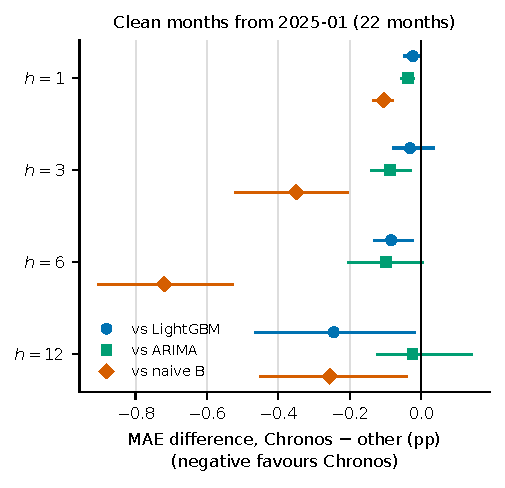
\includegraphics[width=\linewidth]{figures/fig_chronos_accuracy.pdf}
\caption{Point accuracy of Chronos relative to the other forecasters by horizon. Claims are limited to the 22 target months from 2025-01; earlier months are flagged as possibly seen in pretraining.}
\label{fig:chronos}
\end{figure}

\subsection{Other analyses}\label{sec:other}

\paragraph{Post-2025-06 months of the 13 countries (not used).} The run evaluating the design countries on target months from 2025-07 has eleven contributing countries (Nigeria ends in 2024-12 because of the CPI break; Russia has no usable stretch after 2022-03), each with at most 16 months. With blocks of 12 it is degenerate (confidence limits coincide with the estimate, $p$-values sit at the resampling floor) and is not used for any claim; pooled ACI coverage is 0.904, 0.922 and 0.940 at $h=1,3,6$, and no conclusion is drawn.

\paragraph{Exploratory stress and Kazakhstan.} The secondary exchange-rate stress analysis (exploratory sample only; top-decile coverage of ACI 0.849 at $h=3$ against about 0.87 to 0.98 in other deciles, roughly two standard errors, non-monotone) and the post hoc descriptive analysis of Kazakhstan alone (S6, one design country with about 137 origins; no mechanism isolated) are documented in the repository and not repeated here; no stress result exists for the hold-out panels and no confirmatory claim about stress or Kazakhstan is made.
